\subsection{Pipelineknoten}
% Hier musste ich leider manuell skalieren, um zu vermeiden dass das Ummel die ganze Seite einnimmt	
\begin{center}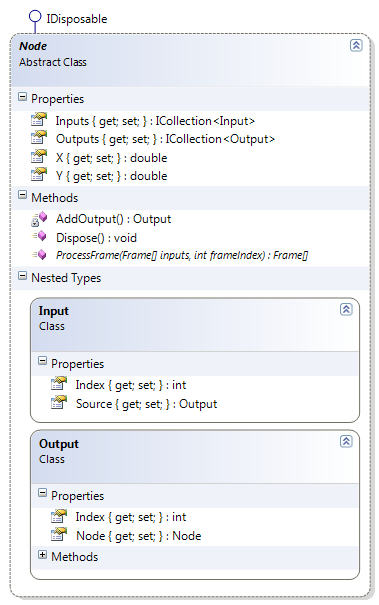
\includegraphics[scale=0.7]{YuvKA.Pipeline/node.png} \\
UML-Klassendiagramm der Basisklasse \name{Node} von der alle Eingabe-, Manipulations- und Ausgabeknoten abgeleitet sind. Auch dargestellt sind die beiden internen Klassen \name{Input} und \name{Output}
\end{center}

\subsubsection{YuvKA.Pipeline.Node}

\begin{verbatim}
[InheritedExport]
[DataContract]
public abstract class Node : IDisposable
\end{verbatim}

\paragraph{Beschreibung}~\\
Die Klasse \name{Node} stellt die gemeinsame Struktur aller Knoten zur Verfügung. Die allgemeine Arbeitsweise eines solchen Knotens besteht darin, dass er nach seiner Konstruktion und dem Hinzufügen seiner Ausgänge durch einen Aufruf der Funktion \name{Processframe} zur Verarbeitung der gegebenen \name{Frame}s ab dem gegebenen Index gebracht wird.

\paragraph{Typmember}
\begin{itemize}

\property{X}
	\begin{verbatim}
	[Browsable(false)]
	[DataMember]
	public double X { get; set; }
	\end{verbatim}
	%<Membererklärung>
	==Hier bitte gute Rechtfertigung wieso ein Knoten seine Position wissen muss.==

%[etc.]

\method{ProcessFrame}
	\begin{verbatim}
	public abstract Frame[] ProcessFrame(Frame[] inputs, int frameIndex);
	\end{verbatim}
	Verarbeitet die gegebenen \name{Frame}s entsprechend des internen Algorithmus' und gibt ein Array von \name{Frame}s als Resultat zurück.

%[etc.]

\end{itemize}

%\subsubsection{<weitere Klasse im gleichen Format...>}
%Beschreibung, Member und Methoden, etc.

